\documentclass[a4paper,10pt]{article}
\usepackage{amssymb,amsmath ,amsthm, graphicx}
\usepackage[left=2cm,top=2cm,right=2cm,bottom=2cm,nohead,nofoot]{geometry}
\usepackage{enumitem}

\usepackage[utf8]{inputenc}
\usepackage{amsfonts,amsmath,amssymb,array}

%\addtolength{\voffset}{-1cm}
%\addtolength{\hoffset}{-2cm}
%\addtolength{\textwidth}{4cm}
%\addtolength{\textheight}{2cm}

\newcommand{\lp}{\left(}
\newcommand{\rp}{\right)}
\newcommand{\lrp}[1]{\lp #1 \rp}
\newcommand{\lrb}[1]{\left[ #1 \right]}
\newcommand{\ra}{\rightarrow}
\newcommand{\la}{\leftarrow}
\newcommand{\ds}{\displaystyle}

% MATH ABBREVS
\newcommand{\eps}{\varepsilon}
\newcommand{\inv}{^{-1}}
\providecommand{\gam}{\gamma}
\providecommand{\lam}{\lambda}

% OPERATORS AND KEYWORDS
\newcommand{\kron}{\ensuremath{\otimes}}
\newcommand{\eoe}[2]{ \ve_{#1} \kron \ve_{#2} }
\newcommand{\Del}{\partial}
\DeclareMathOperator{\ave}{ave}
\DeclareMathOperator{\supp}{supp}
\DeclareMathOperator{\cut}{cut}
\DeclareMathOperator{\vol}{vol}
\DeclareMathOperator{\rank}{rank}
\DeclareMathOperator{\nullity}{nullity}
% \DeclareMathOperator{\exp}{exp}
\DeclareMathOperator{\diag}{diag}
\DeclareMathOperator{\tr}{tr}
% \DeclareMathOperator{\min}{min}
% \DeclareMathOperator{\max}{max}

% VECTORS
\providecommand{\vecn}[1]{\ensuremath{\textbf{#1}}}
\providecommand{\hvv}[1]{\hat{\vecn{#1}}}

\providecommand{\va}{\vecn{a}}
\providecommand{\vb}{\vecn{b}}
\providecommand{\vc}{\vecn{c}}
\providecommand{\vd}{\vecn{d}}
\providecommand{\ve}{\vecn{e}}
\providecommand{\vf}{\vecn{f}}
\providecommand{\vg}{\vecn{g}}
\providecommand{\vh}{\vecn{h}}
\providecommand{\vp}{\vecn{p}}
\providecommand{\vq}{\vecn{q}}
\providecommand{\vr}{\vecn{r}}
\providecommand{\vs}{\vecn{s}}
\providecommand{\vu}{\vecn{u}}
\providecommand{\vv}{\vecn{v}}
\providecommand{\vw}{\vecn{w}}
\providecommand{\vx}{\vecn{x}}
\providecommand{\vy}{\vecn{y}}
\providecommand{\vz}{\vecn{z}}
\providecommand{\vlam}{\boldsymbol{\ensuremath{\lambda}}}

% MATRICES
\newcommand{\pmat}[1]{\begin{pmatrix} #1 \end{pmatrix}}
% \newcommand{\bmat}[1]{\lrb{ \begin{array}{c} #1 \end{array} }}
\newcommand{\bmat}[1]{ \begin{bmatrix} #1 \end{bmatrix} }

\newcommand{\spmat}[1]{\left(\begin{smallmatrix} #1 \end{smallmatrix}\right)}
\newcommand{\sbmat}[1]{\left[\begin{smallmatrix} #1 \end{smallmatrix}\right]}

\providecommand{\matbld}[1]{\ensuremath{\textbf{#1}}}
\providecommand{\mA}{\matbld{A}}
\providecommand{\mB}{\matbld{B}}
\providecommand{\mC}{\matbld{C}}
\providecommand{\mD}{\matbld{D}}
\providecommand{\mE}{\matbld{E}}
\providecommand{\mF}{\matbld{F}}
\providecommand{\mG}{\matbld{G}}
\providecommand{\mH}{\matbld{H}}
\providecommand{\mI}{\matbld{I}}
\providecommand{\mJ}{\matbld{J}}
\providecommand{\mL}{\matbld{L}}
\providecommand{\mM}{\matbld{M}}
\providecommand{\mN}{\matbld{N}}
\providecommand{\mP}{\matbld{P}}
\providecommand{\mQ}{\matbld{Q}}
\providecommand{\mR}{\matbld{R}}
\providecommand{\mS}{\matbld{S}}
\providecommand{\mT}{\matbld{T}}
\providecommand{\mU}{\matbld{U}}
\providecommand{\mV}{\matbld{V}}
\providecommand{\mW}{\matbld{W}}
\providecommand{\mX}{\matbld{X}}
\providecommand{\mY}{\matbld{Y}}
\providecommand{\mZ}{\matbld{Z}}

\providecommand{\mLam}{\boldsymbol{\ensuremath{\Lambda}}}

\usepackage{csquotes}
\usepackage{booktabs} 
% \usepackage{paralist} % for compactenum

%kyle's macros

\DeclareMathOperator{\tw}{tw}

\providecommand{\vvk}[2]{\vecn{#1}^{(#2)}}
\providecommand{\hvf}{\hvv{f}}

\newtheorem{theorem}{Theorem}
\newtheorem{lemma}{Lemma}
\newtheorem{corollary}{Corollary}
\newtheorem{proposition}{Proposition}


%% MAIN TEXT
\title{Network analysis preliminaries:\\
Graph theory and linear algebra}
\author{Kyle Kloster}


\begin{document}
\maketitle

\abstract{
Basic graph and matrix definitions, ideas, tools and facts.
 }


 %%%%%%%
 %%%%%%%
 %%%%      SECTION HEADING
 %%%%%%%
 %%%%%%%
\section{Overview}
This document summarizes the relevant terminology, ideas, and tools to dig into some network analysis. We're particularly interested in graph structures and sparsity (like cliques and k-cores), and their relationship to graph-matrix objects (like functions of the adjacency matrix and eigenvalues of the Laplacian). We'll define and discuss these terms (and many more) in the sections to come.

As with many subjects there is a wealth of terminology to cover at the start -- if it feels overwhelming, or unmotivated, don't worry. It is abstract and there is a bit much of it, but as we use the definitions and notation more and more, it will become easier. All of the terms here will be re-used a lot as we study and discuss objects and problems with neat theory and applications.

%%%%%%%
%%%%%%%
%%%%      NOTATION AND DEFINITIONS
%%%%%%%
%%%%%%%
\section{Notation and definitions}\label{sec:notation}
%%%
%%% DEFINITIONS
%%%
\subsection{Graph basics}\label{sec:notation:graph}
Throughout, let $G = (V,E)$ be a graph with nodes (vertices) $V$ and edges (links) $E$. We let $n = |V|$ and $m = |E|$. We label the nodes with integers 1 through $n$ and can refer to a node $v_j$ by its integer label $j$. We identify an edge by its endpoints $i$, $j$, and label it $e_{ij}$. The \emph{degree} of a node is the number of edges touching that node, and we denote it $d(j)$ or $d_j$.
A graph is \emph{simple} if no nodes have more than one edge between them (i.e. no multi-edges). A graph is \emph{loopless} if no node has a \emph{self edge} (an edge that has the same node for both of its endpoints). A graph is \emph{undirected} if no edge has a direction, and is \emph{directed} otherwise. A graph is \emph{weighted} if either the nodes or edges have scalars $e \in \mathbb{R}$ associated with them; a graph is \emph{unweighted} otherwise (in which case all edges are assumed to have weight 1).

Unless otherwise stated, we deal entirely with graphs that are simple, loopless, undirected, and unweighted. Because this setting is the one most often considered by most studies, we will call such a graph a \emph{standard} graph. We will also usually deal with graphs that are \emph{connected} (defined below).

%%%
%%% CONNECT
%%%
\subsection{Connectivity basics}\label{sec:notation:connect}
A \emph{walk} from node $i$ to node $j$ is a sequence of nodes starting with $s$ and ending with $t$ such that consecutive nodes in the sequence, $v_{j}$ and $v_{j+1}$, are connected by an edge. Intuitively: imagine standing on a node $y$ in $G$, then picking an edge that touches your node, and stepping across that edge. Then repeat. Any node $v$ that you land on, you have arrived via a walk from $y$ to $v$.

Note that a walk from $s$ to $t$ is allowed to step across any edge or node multiple times.
%A \emph{trail} is a walk that does not repeat any edges. Think of a trail in a park -- it might lead you back to the same intersection place but would not have you re-trace steps along a particular road. (Trails are not discussed as often as walks or our next object, paths.)
A \emph{path} is a walk that does not repeat any nodes, except possibly the final node, i.e. a path could begin at node $v$ and ends at node $v$. Any walk or path that begins and ends at the same node is called \emph{closed}.

A graph $G$ is \emph{connected} if for every pair of nodes $u,v$ in $V$ there exists a path between nodes $u$ and $v$. Any graph $G$ can be divided into \emph{connected components} $G_1, \cdots, G_c$, i.e. subgraphs of $G$ such that all nodes of $G$ are contained in the node-sets of $G_j$, and each subgraph $G_j$ is a connected graph. (Then no edges would connect nodes in subgraphs $G_i, G_j$ with $ i \neq j$.) The graph consisting of a single node is considered a single connected component.

An \emph{edge cut-set} $S$ of a graph $G$ is a set of edges such that if remove all edges from $G$, the resulting graph $G'$ will one more connected component than $G$. In particular, if $G$ is a connected graph, then an edge cut-set $S$ is a set of edges such that deleting those edges will separate (split, disconnect) $G$ into two connected components.

%%%
%%% MATRIX
%%%
\subsection{Matrix and vector basics}\label{sec:notation:matrix}

In general we use non-bold letters $(a,b,c,\lambda, x, \gamma)$ to represent scalars, and bold letters to denote arrays/vectors/matrices. Lower-case bold letters indicate vectors, e.g.
$\ve,\vv,\vx, \vlam$,
whereas upper-case bold letters indicate matrices, $\mA, \mM, \mX, \mLam$. To refer to a specific vector entry, we might use any of $\vx(j), \vx[j], (\vx)_j, x(j), x[j], x_j$. To refer to entry $i,j$ of a matrix $\mA$, we use $A(i,j)$, $A_{i,j}$, or $(\mA)_{i,j}$. We denote the transpose of a matrix $\mM$ by $\mM^T$.

The dimension of any vector and matrix can usually be inferred from the context if it is not specifically stated. When dealing with a graph on $n$ nodes, most vectors are $n \times 1$ (i.e. we use column vectors) and most matrices are $n \times n$, though occasionally there are matrices whose dimensions are determined by some quantity other than the number of nodes, for instance the number of edges.
There are a handful of specific letters that we reserve for specific objects: the vector $\ve$ denotes the vector of all 1s; the vectors $\ve_j$ are standard basis vectors, meaning they are all 0s except with a 1 in the $j$th entry. The matrix $\mI$ is the $n\times n$ identity matrix, $0$ is used to denote the zero vector and the zero matrix, and $\mJ$ denotes a matrix of all 1s.

To any $n$-node graph $G = (V,E)$ we can associate the graph's \emph{adjacency matrix}, usually denoted $\mA$: it is an $n \times n$ matrix in which row $j$ and column $j$ each encode the edge-information of node $j$. More specifically, the matrix satisfies $\mA_{i,j} = 1$ iff nodes $i$ and $j$ are connected by an edge. Then $\mA_{i,j} = 0$ otherwise. Note that this matrix is symmetric, since entries $\mA_{i,j}$ and $\mA_{j,i}$ are both ``1" when nodes $i$ and $j$ are connected by an edge.

We use $\vd$ to denote the $n\times 1$ vector of degrees, so that $\vd_j = d(j)$, and we use $\mD$ to denote the diagonal \emph{degree matrix}, $\mD = \diag(\vd)$. Then we can define the \emph{Laplacian matrix} (also called the \emph{combinatorial Laplacian}, \emph{discrete Laplacian}, and \emph{Kirchoff matrix}) to be $\mL = \mD - \mA$.

The \emph{edge-node incidence matrix} (which we call simply the \emph{incidence matrix}) of a graph that has $m$ edges and $n$ nodes is the $m \times n$ matrix $\mB$ that has $\mB(i,j) = \pm1$ iff edge $i$ has node $j$ as one of its endpoints. To be more precise about the sign of the entries, let edge $i$ have node endpoints $j_{1}$ and $j_{2}$ and label those nodes so that $j_1 < j_2$. Then $\mB(i,j_1) = -1$ and $\mB(i,j_2) = 1$. You can think of this as every edge pointing from its endpoint with smaller label to its endpoint with larger label, so that the edge is negative (outgoing) at the smaller label $j_1$ and positive (ingoing) at the larger label node.

Don't get caught up in these details, but to be totally correct, these details ought to be mentioned:
(Note that we know the labels of the two nodes are not equal, because we assumed our graph is loopless, and so no node can be both endpoints of a single edge. Since the edge endpoints are distinct nodes, we know one of the two must have a larger label, and hence we can assume $j_1 < j_2$). Also, this particular way of assigning signs to the entries of matrix $\mB$ is one coherent way to assign $\pm1$ entries, but it turns out you can assign the signs in almost any way, as long as each edge has exactly one positive and one negative endpoint, and the important results will all still hold for the matrix $\mB$.

\subsection{Exercises}

\begin{enumerate}[label=\ref{sec:notation}.\arabic*]
\item Prove that for any standard graph, the sum of the degrees of all nodes equals twice the number of edges, i.e. $\sum_{v \in V} d(v)  =  2|E|$.

\item Let $G$ be a standard graph with $n>1$ nodes. Is it possible that all $n$ nodes have distinct degrees, i.e. is it possible that no two nodes have the exact same degree? If yes, give an example, if no prove that it is impossible.

\item Let $G$ be a connected, standard graph. Prove that deleting a single edge, $e$, from $G$ cannot disconnected $G$ into more than two connected components. In other words, suppose that deleting $e$ from $G$ produces the disconnected graph $G' = G -\{e\}$; show the number of connected components is 2.

\item\label{sec:notation:problem-volume} Let $G$ be a standard graph with adjacency matrix $\mA$. Prove that $\vd = \mA \ve$. Prove that $\ve^T\mA\ve = 2 |E|$.

\item\label{sec:notation:problem-laplacian-singular} Let $G$ be a standard graph with Laplacian matrix $\mL = \mD - \mA$. Prove that $\mL\ve = 0$ using problem \ref{sec:notation:problem-volume}.

\item\label{sec:notation:problem-laplacian-incidence-decomposition} Let $G$ be a standard graph with incidence matrix $\mB$ and Laplacian matrix $\mL$. Prove that $\mL = \mB^T\mB$. Now prove that $\mL\ve = 0$ using the fact that $\mL = \mB^T\mB$.

\end{enumerate}


%%%%%%%
%%%%%%%
%%%%      SECTION HEADING
%%%%%%%
%%%%%%%
\section{Network Analysis Fundamentals}\label{sec:fundamentals}


\subsection{Eigen-fundamentals}\label{sec:fundamentals:eigen}

Eigen-information of graph-related matrices turns out to be a powerful tool in analyzing structural information of graphs. For example, we will see that the second smallest eigenvalue of the Laplacian matrix of a graph gives information about the best cut we can find in the graph. In a broader setting, the eigen-information of a matrix provides powerful tools for faster matrix operations and can even be used for data compression.


Let $\mM$ be any $n \times n$ matrix with entries over the real numbers $\mathbb{R}$. A vector $\vv$ is an \emph{eigenvector} of $\mM$ with \emph{eigenvalue} $\lam$ iff $\mM\vv = \lam \vv$. We call the tuple $(\vv, \lam)$ an \emph{eigen-pair}. Suppose the matrix $\mM$ has $n$ eigenvectors $\vv_j$ with eigenvalues $\lam_j$. Set $\mV = [\vv_1, \cdots, \vv_n]$ and $\mLam = \diag(\lam_1, \cdots, \lam_n)$. Then we have that the equation
\[
\mM\mV = \mV\mLam
\]
holds column-wise by definition of the columns $\vv_j$ being eigenvectors of $\mM$ (verify this). Note that the matrix $\mV$ is invertible iff the $n$ eigenvectors $\vv_j$ are linearly independent; if they are, we can then rearrange the above equation to yield the \emph{diagonalization} of matrix $\mM$, also called the \emph{spectral decomposition} or \emph{eigen decomposition} of matrix $\mM$:
\begin{equation}\label{eqn:spectraldecomposition}
\mM = \mV \mLam \mV\inv.
\end{equation}
If a matrix $\mM$ has a diagonalization, we say it is \emph{diagonalizable}. When discussing eigenvalues of a matrix, we give the following conventional ordering to the eigenvalues: $\mM$ has eigenvalues \[\lam_1 \geq \lam_2 \geq \cdots, \geq \lam_{n-1} \geq \lam_n.\]

The following theorem guarantees that adjacency matrices of undirected graphs always have a nice diagonalization:
\begin{theorem}\label{thm:symmetric-diagonalizable}
  Let $\mM \in \mathbb{R}^{n \times n}$ be a symmetric. Then $\mM$ has $n$ linearly independent eigenvectors $\vv_j$, and so we can express $\mM = \mV \mLam \mV\inv$.
\end{theorem}
Since undirected graphs (and, in particular, standard graphs) have symmetric adjacency matrices $\mA$, we can always make use of the diagonalization of $\mA$ and $\mL$.

Recall that the \emph{rank} of a matrix is equal to (1) the dimension of the columnspace of $\mM$, (2) the dimension of the rowspace of $\mM$.
\begin{proposition}
  If $\mM$ is a diagonalizable, then $\rank(\mM)$ is equal to the number of nonzero eigenvalues $\lam_j \neq 0$ of $\mM$, which equals the number of linearly independent eigenvectors $\vv_j$ of $\mM$.
\end{proposition}

\begin{proposition}\label{thm:rank-invertible}
  An $n\times n$ matrix $\mM$ is invertible iff $\rank(\mM) = n$.
\end{proposition}

An eigenvalue $\lambda$ of a matrix $\mM$ can have multiple linearly independent eigenvectors associated with it. The most straightforward example is the $n \times n$ identity matrix $\mI$, which has the eigenvalue 1 with $n$ different linearly independent eigenvectors; for exaxmple, each standard basis vector $\ve_j$ is an eigenvector of $\mI$, since $\ve_j = \mI\ve_j$.
If an eigenvalue $\lam$ of $\mM$ has multiple lienarly independent eigenvectors, then those eigenvectors generate a subspace, called an \emph{eigenspace} associated with the eigenvalue $\lam$. For Egienvalue $\lam_j$, let $E_j$ denote the subspace of all eigenvectors $\vv$ with eigenvalue $\lam_j$, i.e. all vectors $\vv$ such that $\mM\vv = \lam_j \vv$. Then the dimension of the subspace $E_j$ is defined to be the \emph{geometric multiplicity of the eigenvalue} $\lam_j$. If a matrix has 0 as an eigenvalue, this is so important that we give a special name to the multiplicity of the eigenvalue 0 -- if a matrix $\mM$ has eigenvalue 0 with geometric multiplicity $m_0$, then we say $\mM$ has \emph{nullity} $m_0$, which we will denote $\nullity(\mM)$.
This brings us to the ``Rank-nullity theorem", which has a useful connection to Proposition~\ref{thm:rank-invertible}:
\begin{theorem}[Rank-nullity]
  For any $\mM \in \mathbb{R}^{n \times n}$ the rank and nullity of $\mM$ satisfy $\rank(\mM) = n - \nullity(\mM)$. In particular, $\mM$ is invertible iff $\nullity(\mM) = 0$, i.e. 0 is not an eigenvalue of $\mM$.
\end{theorem}

Finally we connect these concepts to our analysis of networks, by looking more closely at Exercise~\ref{sec:notation:problem-laplacian-singular} from the previous section.
First, we restate the exercise as a result:
\begin{proposition}
Let $\mL$ be the Laplacian of a standard graph. Then $\mL$ has eigenvalue $\lam = 0$ with multiplicity at least 1, and $\ve$ as an eigenvector: $\mL\ve = 0\ve$.
\end{proposition}
This means Laplacian matrices are never invertible, since they always have nullity at least 1. However, something neat happens if we look more closely at this result.
But we'll get there -- first, we need one more preliminary result.
\begin{lemma}
  Let $G$ be a standard graph with $k$ connected components, $G_1, \cdots, G_k$, with connected component $G_j$ having Laplacian matrix $\mL_j$. Then the graph $G$ can have its nodes ordered so that the Laplacian matrix $\mL$ of $G$ is
  \[
\mL = \diag( \mL_1, \cdots, \mL_k ) = \bmat{\mL_1 & & \\  & \ddots &  \\  &  &  \mL_k}.
  \]
\end{lemma}
This lemma makes it easier to prove the following theorem, which gives us a first glimpse of how Linear Algebra can provide information useful to Graph Theory:
\begin{theorem}
  Let $G$ be a standard graph with $k$ connected components, and with Laplacian matrix $\mL$. Then $k = \nullity(\mL)$.
\end{theorem}
In words, the multiplicity of zero as an eigenvalue of $G$'s Laplacian matrix is the same as the number of distinct connected components of $G$.


%\subsection{Structure inherent to graph matrices}\label{sec:fundamentals:graphstructure}

There are a lot of nice properties that matrices and their eigenvalues/vectors can have if the matrices are ``well-behaved" in a sense. It turns out, many graph matrices enjoy a lot of these nice properties! Here we discuss some of the most useful of these properties. What do we mean by well-behaved? Think of polynomials -- the polynomial p(x) = x^2-1 is very well-behaved in the sense that all of its rooots are integers; in contrast, a polynomial like p(x) = x^2 + 2 has roots that are complex numbers with irrational components ($\sqrt{2}$). This is not a perfect analogy but it gives the intution that a ``well-behaved" object is easier to work with. Next we cover two examples of what we mean for matrices to be well-behaved in our context.

\begin{proposition}
  Let $G$ be a standard graph with incidence matrix $\mB$ and Laplacian matrix $\mL$. Then $\mL = \mB^T\mB$.
\end{proposition}


\subsection{Graph walks, graph matrices}\label{sec:fundamentals:walks}


Here we look at what I call the Fundamental Lemma of Network Analysis because of how often it is used.
\begin{lemma}[Fundamental Lemma of Network Analysis]\label{thm:fundamental-walk}
Let the graph $G$ have adjacency matrix $\mA$. Then the number of length $k$ walks from node $i$ to node $j$ is equal to $(\mA^k)_{ij}$.
\end{lemma}

This lemma is so often used because it gives us a way to measure connectivity between different nodes -- it gives us a way to measure, for a fixed node $s$, what nodes are most important to, or similar to, the node $s$?
Consider the polynomial $p(x) = \sum_{k=1}^N x^k$. Then the vector
\[
\vf =  p(\mA)\ve_s = \sum_{k=1}^N (\mA^k)\ve_s
\]
tells us for each node $j$ in the graph, how many total walks are there from node $s$ to node $j$ of length $\leq N$ ?
Large entries in the vector $\vf$ end up being good predictors for nodes that are important to node $s$.






\subsection{Exercises}

\begin{enumerate}[label=\ref{sec:fundamentals}.\arabic*]
\item Prove Lemma~\ref{thm:fundamental-walk}. Hint: begin with $\mA^1$ as the base case, and proceed by induction. For the case $(\mA^k)_{ij}$, think about the question ``how do you make a walk from node $i$ to node $j$ that is of length $k$?".

\end{enumerate}



\section{More on structured sparsity}\label{sec:structured-sparsity}


Here we begin our forray into notions of structured sparsity. We start with one of the simpler notions, that of the \emph{degeneracy} of a graph $G$, which the Theory in Practice Lab has described as follows:
``No good notion of sparsity \emph{doesn't} imply bounded degeneracy." In other words, any good idea of $G$ having structured sparsity should imply that $G$ has bounded degeneracy. Next, we explore exactly what that means.


\subsection{Degeneracy and k-cores}\label{sec:degeneracy}

As usual, all graphs we consider here are standard graphs.
A \emph{$k$-core} is a graph in which every node had degree at least $k$. A $k$-core of a graph $G$ is any induced subgraph of $G$ that is also a $k$-core.
The \emph{$k$-core number of a node} $v$ in $G$ is the largest number $k$ for which $v$ is contained in a $k$-core of $G$.
The \emph{$k$-core of $G$} is the largest number $k$ for which $G$ has a $k$-core;
the $k$-core number of $G$ is also called the \emph{degeneracy} of $G$.


\subsubsection{Uses and Examples}

Degeneracy provides a much more useful notion of ``density" than, say, maximum degree or average degree.
For example, a star graph on $n$ nodes is a very sparse graph, yet it has maximum degree $n-1$, which ``sounds like it might be dense". In contrast, the degeneracy of a star is always 1, which reveals its  true sparsity.
Similarly, if a graph has constant average degree it does not guarantee any useful bound on the maximum clique size: an $n$ node graph with $kn$ edges can have a clique of size $\sim \sqrt{(k-1)n}$ (by constructing a path graph on $n$ nodes, then putting all other edges in a clique).
In contrast, the degeneracy of such a graph would be lower-bounded by the clique size, because a $k$-clique is always a $(k-1)$-core.

We could also think about this from the other direction, i.e. that the core number (degeneracy) of $G$ always gives a bound on the max clique number.
These bounds are not always useful, though: there are graphs with arbitrarily large gaps between the max-clique size and $k$-core number.
For example, a hypercube on $2^n$ nodes is always an $n$-core, but the largest clique is always of size 2.

Another useful feature related to degeneracy and core numbers is the idea of a \emph{degeneracy ordering} of a graph's nodes. This is any ordering on the nodes of $G$ that sorts the nodes, in ascending order, according to the nodes' $k$-core numbers. It is called the degeneracy ordering because if you delete these nodes, one-by-one, according to this ordering, then the core number of node $v$ is exactly equal to the degree of $v$ at the time $v$ is deleted. A degeneracy ordering can be useful for processing the nodes and edges of a graph in an efficient way.

For a linear-time algorithm that computes the $k$-core numbers of all nodes in $G$, see~\cite{batagelj2003m}. To use $k$-cores to accelerate computation of the max-clique in a graph, see~\cite{rossi2014fast}.

\subsubsection{Exercises}\label{sec:degeneracy:exercises}

\begin{enumerate}[label=\ref{sec:degeneracy}.\arabic*]
  \item If $G$ has maximum degree $d$, prove that degeneracy of $G$ is bounded above by $d$.
  \item If $G$ has degeneracy $k$, does this imply any upper bound on the number $n$ of nodes in the graph?
  For a fixed number of nodes $n$, does degeneracy $k$ imply an upper bound on the number of edges?
  \item If $G$ has degeneracy $k$, does this imply any lower bound on the number $n$ of nodes in the graph?
  For a fixed number of nodes $n$, does degeneracy $k$ imply a lower bound on the number of edges?
\end{enumerate}

\subsection{Tree-decompositions and tree-width}\label{sec:tree-decomposition}

% Merely having bounded degeneracy is not always enough to ensure that a difficult problem can be easily solved on a graph $G$. For example, computing the \emph{chromatic number} of a graph (i.e. the smallest number of colors necessary to color the vertices of $G$)
\paragraph{Definition}
We will, eventually, give a formal definition of a tree-decomposition of a graph $G$, but first we want to approach the topic intuitively.
A tree-decomposition is not ``a decomposition of a graph into trees" (this idea is closer to the \emph{arboricity} of a graph). Rather, a tree-decomposition is a map from the nodes of $G$ to some tree $T$ such that each node of $T$ (which we call a ``bag" and usually denote by $X_j$) contains a set of vertices of $G$, and we can think of $T$ as being a map of $G$ that tells us ``how to process the nodes of $G$ in an efficient order". Let's take the simplest possible type of tree for $T$, a path. If we have a tree-decomposition of $G$ such that its nodes are all mapped into bags of $T$ that are lined up in a path ($X_1, X_2, \cdots, X_k$), then to solve a problem on the entire graph $G$ it can suffice to simply perform computations on the nodes of $G$ one bag $X_j$ at a time before moving on to the next bag $X_{j+1}$.
To show why the tree-decomposition can be useful as a ``processing map", we next describe it more rigorously.

Formally, a \emph{tree-decomposition} of a graph $G = (V,E)$ consists of a tree $T = (V_T,E_T)$ whose nodes we call ``bags", such that:
\begin{enumerate}[label=T.\arabic*]
  \item Every node of $G$ is contained in at least one bag $X_j$ of $T$.
  \item Every edge of $G$ has both its endpoints contained in at least one bag $X_j$ of $T$.
  \item\label{def:tree-decomp:bag-rule} For each node $v$ in $G$, the set of bags $X_{j} \in V_T$ containing $v$ induces a connected subtree of $T$.
\end{enumerate}

Any such mapping from $G$ to a tree $T$ that satisfies these properties is a tree-decomposition of $G$; a given graph can have many tree-decompositions. For a given tree decomposition, we define the \emph{width} of the decomposition to be $\max_{X_j \in V_T}  (|X_j| - 1 )$. The \emph{tree-width} of the graph $G$, $\tw(G)$, is then the minimum width of all tree-decompositions of $G$.

\paragraph{Understanding its usefulness}
The basic idea of the usefulness of a tree decomposition is that the entire graph can be examined by simply examining all nodes in each bag, one bag at a time. If the graph has low tree-width, then no big is too large, and so each bag can be swiftly processed. Thus, ``graphs with bounded tree-width" is a class of structurally sparse graphs for which there exist a lot of fixed-parameter tractable algorithms, where the parameter that gets fixed is the tree-width of the graph, $\tr(G) = k$.

Tree-decompositions also have connections to vertex seperators. A \emph{vertex separator} of a connected graph $G = (V,E)$ is a set $S \subset V$ of nodes such that deleting $G - S$ is disconnected.
Vertex separators can be very useful in divide-and-conquer style algorithms, and in distributing graphs across multiuple processors for more efficient computation or storage.
It turns out that each bag $X_j$ in any tree decomposition of $G$ is a vertex separator.

An \emph{edge separator} of a connected graph $G = (V,E)$ is a set $F\subset E$ of edges such that $G-F$ is disconnected. This is also called an \emph{edge cut} or simply a \emph{cut}.
A cut, or edge separator $F$, is ``balanced" if deleting $F$ leaves behind two graph components that are not too different in size (this is a hand-wavey, intuitive term, not a rigorous once). To be more precise, we define the \emph{conductance} of a cut as follows. First note that any cut $F$ necessarily splits the set of nodes into two components,  $S$ and $G-S$. So, we can define a cut either by its edge set, $F$, or, equivalently, by the set of nodes that it disconnects, $F = \cut(S,G-S)$. Recalling that $\vol(S)$ is defined to be the sum of the degrees of the nodes in $S$, $\vol(S) = \sum_{v \in S} d(v)$, we can now define the condutance of the cut (edge separator) $F = \cut(S,G-S)$ to be
\begin{equation}\label{eqn:def:conductance}
  \text{conductance}(S) = \frac{\cut(S,G-S)}{\min\{ \vol(S), \vol(G-S) \} },
\end{equation}
which is conventionally denoted $\phi(S)$.
Note that condutance is always between 0 and 1; when $\phi(S) = 0$, the cut is very small because $S$ is not connected to the rest of $G$ (so the cut contains zero edges), whereas when $\phi(S) = 1$ the cut is larger, because all edges connected to nodes in $S$ leave the set $S$ and have their other endpoints in the set $G-S$ (so the cut contains a ``maximal" number of edges).

The connection of topics here is that every cut (edge separator) containing $t$ edges guarantees the existence of a vertex separator that contains no more than $t$ nodes. To see this, note that a cut $F = \cut(S,G-S)$ containing $t$ edges is incident to no more than $t$ nodes in $S$ (and no more than $t$ nodes in $G-S$). Thus, deleting those $s \leq t$ nodes will separate the graph into two pieces, and so some subset of the nodes in $S$ is a vertex separator.

\begin{proposition}
  Every cut (edge separator) in $G$ yields at least one vertex separator.
\end{proposition}

This provides a direct connection from conductance and cuts to vertex separators and, hence, tree-decompositions.
Thus, we next move our focus to eigenvalue approaches to understanding conductance and cuts in a graph.
Keep in mind that the benefit of tree decompositions is not the size of the tree $T$, but the width of the bags associated with the tree -- in other words, a tree decomposition is most helpful if all of the vertex separators it provides are small separators (contain a small number of nodes).


\subsubsection{Exercises}\label{sec:tree-decomposition:exercises}

\begin{enumerate}[label=\ref{sec:tree-decomposition}.\arabic*]
\item Let $G$ be a connected graph with a node $v$ of degree 1. Prove that deleting $v$ from $G$ does not disconnect $G$; i.e. prove that $(G-v)$ is connected.
\item Prove that a tree must have at least one node of degree 1. Then use that result to prove that a tree must have at least two nodes of degree 1.
\item Prove that a connected graph in which every node has degree at least 2 must contain at least one cycle.
\item Prove that every path graph $P$ has a tree-decomposition of tree-width 1. (Hint: take the path on $n$ nodes and tell how to construct construct the bags. (Sub-hint: width 1 means that each bag has exactly two nodes in it.) )
  \item Prove that if $G$ is a tree, then its tree-width is 1. (Hint: tree-width 1 means that the tree decomposition has width 1, which means every bag in that decomposition contains no more than 2 nodes.) (Hint 2: make a couple small trees and explicitly construct tree-decompositions for them with width 1. Notice anything about how each edge of the tree gets mapped to bags in the tree-decomposition? )
  \item Let $G = (V,E)$ be a connected graph. Let $G$ have a tree decomposition with tree $T=(V_T,E_T)$ (i.e. $V_T$ is the set of bags of the tree-decomposition).
  Fix any bag $X_j \in V_T$ and recall that a bag in a tree-decomposition consists of a set of nodes in the original graph, $G$.
  Let $G'$ be the graph that results from deleting from $G$ all nodes $v$ in the bag $X_j$, i.e. let $G' = G-X_j$.
  Prove that $G'$ is disconnected.
  (i.e. prove that each bag of a tree-decomposition for a graph $G$ gives rise to a vertex separator of $G$.)

  \item Prove that rule~\ref{def:tree-decomp:bag-rule} in the definition of tree-decomposition is equivalent to the following: ``for any two bags $X_i, X_j$ in the tree $T$, every bag $X$ on the path in $T$ connecting $X_i$ to $X_j$ must contain their intersection, i.e. $X_i \cap X_j \subseteq X$ ." (i.e. show that we could replace rule~\ref{def:tree-decomp:bag-rule} with this rule, and the resulting definition of tree-decomposition would be equivalent).
\end{enumerate}



This section contains exploring notions of structured sparsity. We will further develop some ideas useful to the study of tree-decompositions and degeneracy.

\subsection{Minor subgraphs}\label{sec:minors}

As usual, all graphs we consider here are standard graphs.
Recall that a graph $G$ contains $H$ as a \emph{minor subgraph} (also called simply ``a minor") if you can obtain a copy of $H$ by a sequence of node deletions, edge deletions, and edge contractions (defined below).
We will later describe important variations on this idea (e.g. ``shallow" and ``topological" minor subgraphs), but first we want to make clear the importance of subgraph minors to the study of sparsity.

We will illustrate the connection of minors to sparsity with an example.
One canonical example of ``sparse" graphs are the family of planar graphs -- planar graphs have $O(n)$ edges and bounded degeneracy.
It turns out that planar graphs are completely characterized by subgraph minors.
To elaborate: a graph $G$ is planar if and only if $G$ does not contains $K_5$ or $K_{3,3}$ as minors (where $K_5$ is the complete graph on 5 nodes, and $K_{3,3}$ is the complete-bipartite graph with 3 nodes in each partition).
This is an example of a type of sparsity that is completely characterized by specific graph minors.

The point here is that having knowledge of the minors of a graph can help determine the sparsity of the graph.
Therefore, we would like an easy way to learn some information about the minors of a graph.
We are not aiming to characterize any graph family completely (that is a little ambitious); rather, our goal is to try to reveal connections between a graph's eigenproperties and a graph's minors.


\subsubsection{Terminology}

%topological minors, and $r$-shallow minors
\paragraph{Operations}

To perform an \emph{edge contraction} on an edge with endpoints $v_1, v_2$, create a new node $v$, attached an edge from $v$ to each neighbor of $v_1$ and each neighbor of $v_2$, then delete nodes $v_1$ and $v_2$. You can think of this as merging the two nodes $v_1, v_2$ into each other.

\begin{figure}[h!]
  \centering
  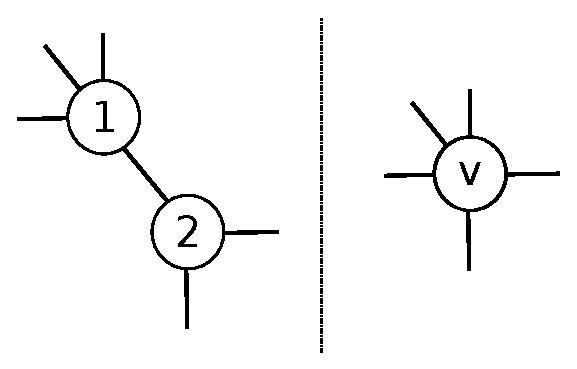
\includegraphics[scale=0.75]{edge-contraction}
  \caption{(\emph{Left}.) Nodes $v_1$ and $v_2$ connected by an edge. (\emph{Right}.) The graph after contracting edge $v_1v_2$, merging nodes $v_1$ and $v_2$ into one new node, $v$.\label{fig:contracting}}
\end{figure}

A \emph{subdivision} (or ``edge subdivision") is sort of the reverse of an edge contraction: given an edge with endpoints $v_1, v_2$, to subdivide the edge $e_{12}$, create a new node $v$, connect $v$ with an edge to node $v_1$ and an edge to $v_2$, then delete edge $e_{12}$. This operation is like spitting edge $e_{12}$ into two pieces connected by a new node $v$. Note that a subdivision introduces a node of degree two. The reverse process, ``un-subdividing", is called \emph{smoothing} or \emph{dissolving} a node of degree two. If node $v$ has degree two and is connected to nodes $v_1$ and $v_2$, then smoothing node $v$ is performed by connecting node $v_1$ and $v_2$ with an edge, then deleting node $v$. See Figure~\ref{fig:smoothing} for an illustration. Smoothing a node of degree two can also be thought of as an edge-contraction on either of the edges touching the node.

\begin{figure}[h!]
  \centering
  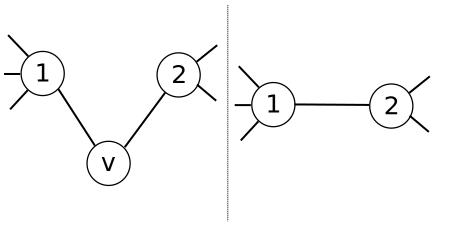
\includegraphics[scale=0.75]{smoothing}
  \caption{(\emph{Left}.) Nodes $v_1$ and $v_2$ separated by a node of degree two, $v$. (\emph{Right}.) The graph after node $v$ has been smoothed; alternatively, this can be understood as contracting edge $v_1v$ or edge $v_2v$.
  Note that viewing the figure from right to left gives an illustration of the edge between $v_1$ and $v_2$ being subdivided.\label{fig:smoothing}}
\end{figure}

A graph $T$ is a \emph{topological minor} of $G$ if you can produce $G$ from $T$ by subdividing edges of $T$, and adding nodes and edges to $T$. Put another way, $T$ is a topological minor (``top-minor" for short) of $G$ if you can produce $T$ from $G$ by deleting nodes and edges, and smoothing nodes (of degree two). Note that all topological minor subgraphs are also minor subgraphs. See Figure~\ref{fig:topminor} for an example of a graph with a $K_4$ as a topological minor.
For contrast, Figure~\ref{fig:minorsubg} displays a graph that does not contain $K_5$ as a subgraph or as a topological minor subgraph (no node has degree 2, so no nodes can be smoothed), but it does contain $K_5$ as a minor subgraph.

\begin{figure}[h!]
  \centering
  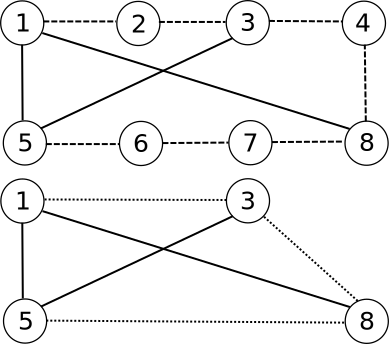
\includegraphics[scale=0.8]{topminor}
  \caption{ In the top graph, smoothing the nodes connected to only dashed egdes yields the graph on bottom as a topological minor. Alternatively, this can be thought of as contracting the dashed edges.
  Note that the dotted edges in the bottom graph indicate the edges produced by the smoothings in the top graph. Finally, viewing this figure from bottom to top, this illustrates an instance of $K_4$ where we then perform several subdivisions on the dotted edges to produce the graph on top.\label{fig:topminor}}
\end{figure}

\begin{figure}[h!]
  \centering
  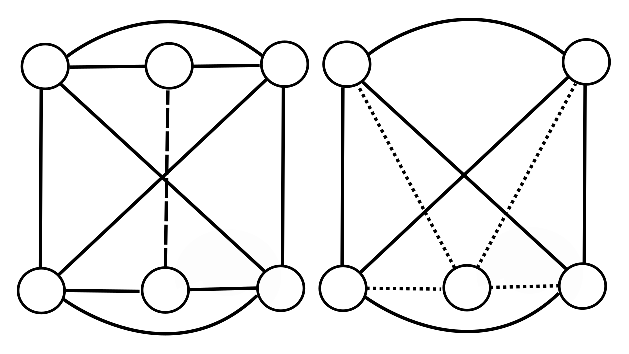
\includegraphics[scale=0.8]{minorsubg}
  \caption{ (\emph{Left}.) This graph does not contain $K_5$ as a subgraph, or as a topological minor subgraph. (\emph{Right}.) Contracting the dashed edge on the left yields a new node, with new dotted edges in the graph on the right. The graph on the right is $K_5$, so this proves the graph on the left has $K_5$ as a minor subgraph.\label{fig:minorsubg}}
\end{figure}

Finally, this brings us to the notion of ``shallowness" of minor subgraphs. Minor subgraphs are used, among other things, for measuring ``density" of a given graph $G$ --- ``$G$ is not sparse" can mean ``$G$ has no dense minor subgraphs like $K_n$". But this notion of measuring density (by looking for the presence of a particular kind of minor subgraph) isn't always precise if, for example, you have to contract a whole lot of sparse components of the graph to be able to produce a ``dense" minor subgraph. The concept of shallowness measures this idea: ``how much contracting must I perform before the result starts to look dense?". We illustrate with an example.

Fix some $n$ and consider $G = K_n$, the complete graph on $n$ nodes; this is the densest graph there is (on $n$ nodes). Now suppose pick one edge and subdivide that edge $c$ times to produce $G'$. There are $\binom{n}{2}$ edges in $G$, so there are $c + \binom{n}{2}$ total edges in $G'$. The graph $G'$ also now has $n+c$ nodes. Is this graph still dense? As we increase $c$ to infinity, $G'$ looks less like ``$G$ with a few extra edges" and more like "one long path graph with a tiny cluster tacked onto its end". Regardless of $c$, the graph $G'$ has $K_n$ as a minor subgraph. But the larger $c$ is, the more contracting must be performed on $G'$ to attain $K_n$ --- the less shallow $K_n$ becomes as a minor subgraph of $G'$.




\begin{tabular}[h]{lcl}
  \\
  object & & operations allowed \\
  \toprule
  minor subgraph & & node deletions \\
    & & edge deletions \\
    & & edge contractions \\
  topological minor subgraph & & node deletions \\
  & & edge deletions \\
  & & node smoothings (contracting edges touching a node of degree 2)\\
  $r$-shallow minor & & node deletions \\
   & & edge deletions \\
   & & ``not more than $r$ edge contractions at each node"\\
\end{tabular}



\section{Eigen-fundamentals, Part 2}\label{sec:fundamentals:eigen2}

Don't worry about this section for a while -- this section will come in handy when we start trying to *prove* things about eigenvalues of certain graphs.



Here we describe some connections of eigenvalue theory to graph cuts and conductance.
Recall that the Laplacian matrix is defined by $\mL = \mD - \mA$, and that it satisfifes $\mL = \mB^T\mB$, where $\mB$ is the edge-node-incidence matrix.
Then we define the \emph{normalized Laplacian matrix} to be $\nmL = \mD^{-1/2}\mL\mD^{-1/2}$,
and we denote its eigenvalues by
\[
\lam_1 \geq \lam_2 \geq \cdots \geq \lam_{n-1} \geq \lam_n.
\]
Defining the \emph{normalized adjacency matrix} to be $\nmA = \mD^{-1/2}\mA\mD^{-1/2}$, note that the normalized Laplacian is simply $\mI - \nmA$.

In this section we will build up to proving a connection of the second smallest eigenvalue of $\nmL$ to the best (smallest) conductance cut in the graph $G$.
We begin by proving a simple but useful fact about the eigenvalues of $\mL$ and $\nmL$.

A $\mM \in \mathbb{R}^{n \times n}$ with all real eigenvalues is \emph{positive definite} iff all of its eigenvalues are positive. Instead, we say $\mM$ is \emph{postive semi-definite} iff all of its eigenvalues are nonnegative.
(Note that all positive definite matrices are positive semi-definite, but a positive semi-definite matrix (which might have eigenvalues equal to 0) is not necessarily positive definite.)

Note that these definitions are restricted to matrices with all real eigenvalues -- the definitions can be extended to matrices with possibly complex eigenvalues, but this is beyond the scope of this project.
(This is because all matrices we are concerned with are similar to symmetric matrices, which are guaranteed to have all real-valued eigenvalues, see Theorem~\ref{thm:symmetric-orthogonal-eigen} below.)

Speaking of symmetric matrices, a particularly well-studied area within positive definite and semi-definite matrices is the subject of symmetric postive definite (SPD) and semi-definite (SPSD) matrices.
So we will have the luxury of dealing in SPD and SPSD matrices here, which enjoy some useful properties that more general postiive (semi-)definite matrices do not. For example:

\begin{theorem}\label{thm:spsd:decomposition}
  Let $\mM \in \mathbb{R}^{n \times n}$ be symmetric. Then $\mM$ is SPSD iff there exists some $\mU \in \mathbb{R}^{n \times r}$ such that $\mM = \mU \mU^T$.
\end{theorem}
\begin{proof}
We will prove only the easier direction of this proposition here. We prove the other direction below, after establishing a little more machinery. Assume that $\mM = \mU\mU^T$, and let $(\vv, \lam)$ be any eigen-pair of the matrix $\mM$, and let $\vv$ be a unit eigen-vector. Then we have
\begin{align}
  \mM\vv &= \lam \vv & \text{definition of eigen-vector} \\
  \vv^T \mM \vv &= \lam \vv^T\vv & \text{left-multiply by $\vv^T$} \\
  \vv^T\mU \mU^T \vv &= \lam & \text{substitute $\mM = \mU\mU^T$ and simplify} \\
  (\mU^T\vv)^T (\mU^T\vv) &= \lam
\end{align}
and since $(\mU^T\vv)^T (\mU^T\vv) \geq 0$, we know that $\lam \geq 0$, proving that $\mM$ is SPSD. This trick will come back to help us a number of times, so keep it in your pocket.
\end{proof}

Recalling that $\mL = \mB^T\mB$, this proposition implies that the Laplacian matrix $\mL$ is positive semi-definite. We also know $\mL$ is symmetric, so $\mL$ is SPSD. Is the Laplacian positive definite? (i.e. not semi-definite?) No: we showed in an earlier section that $\mL\ve = 0\ve$, so we definitely know that $\mL$ is semi-definite, not definite.
But what about $\nmL$? We know it is still symmetric, from its definition.
Furthermore, $\nmL = \mD^{-1/2}\mL\mD^{-1/2} = \mD^{-1/2}\mB^T\mB\mD^{-1/2} = \hat{\mB}^T\hat{\mB}$, where $\hat{\mB} = \mB\mD^{-1/2}$. Thus, $\nmL$ is also SPSD, with nullvector $\vv_n = (\mD^{1/2}\ve)$:
\[
\nmL (\mD^{1/2}\ve) = \mD^{-1/2}\mL\mD^{-1/2} \mD^{1/2}\ve = \mD^{-1/2} \mL\ve = 0 \ve.
\]
With this we have compeleted a proof of the following.
\begin{proposition}
  For any standard graph, $\mL$ and $\nmL$ are SPSD with null-vectors $\ve$ and $\mD^{1/2}\ve$, respectively.
\end{proposition}

We will focus for now on the matrix $\nmL$. Denote its eigenpairs by $(\vv_j, \lam_j)$, and recall that we just finished proving $\lam_1 \geq \lam_2 \geq \cdots \geq \lam_{n-1} \geq \lam_n = 0$.
To continue, we need the following essential result about the eigen-properties of symmetric matrices.

\begin{proposition}\label{thm:symmetric-orthogonal-eigen}
  Let $\mM$ be any real, $n\times n$, symmetric matrix. Then not only is $\mM$ diagonalizable (c.f.~Theorem~\ref{thm:symmetric-diagonalizable}), i.e. $\mM = \mV\mLam\mV\inv$, but we also have that $\mM$ has real eigenvalues and all its eigenvectors are orthogonal, so $\mM = \mV \mLam \mV^T$ and $\mV^T\mV = \mI$.
\end{proposition}

\begin{proof}
We are going to assume Theorem~\ref{thm:symmetric-diagonalizable}, i.e. assume that symmetric $\mM$ has diagonal form $\mM = \mV \mLam \mV\inv$.
Let $\vv_i$ and $\vv_j$ be eigenvectors corresponding to distinct eigenvalues. Claim: then $\vv_i^T\vv_j = 0$. To prove this, note that
\begin{align}
  \lam_i \vv_i^T\vv_j &= (\lam_i \vv_i^T)\vv_j \\
  &= (\vv_i^T \mM^T) \vv_j \\
  &= \vv_i^T (\mM^T \vv_j) \\
  &= \vv_i^T (\mM \vv_j) & \text{because $\mM = \mM^T$} \\
  &= \lam_j  \vv_i^T \vv_j
\end{align}
so that $\lam_i \vv_i^T\vv_j = \lam_j \vv_i^T\vv_j$. If $\vv_i^T\vv_j \neq 0 $, then we can divide both sides by $\vv_i^T\vv_j$ to yield $\lam_i = \lam_j$, but this would contradict the assumption that the eigenvalues were distinct. Thus, $\vv_i^T\vv_j = 0$, proving the claim. Observe that this part of the proof used the fact that $\mM = \mM^T$.

We have proved that eigenvectors of distinct eigenvalues are orthogonal. It remains to show that eigenvectors of the same eigenvalue are orthogonal. For any eigenvalue, $\lam_j$, let $E_j$ be the space spanned by all eigenvectors of $\mM$ associated to $\lam_j$. So for all $\vu$ such that $\mM \vu = \lam_j \vu$, we have $\vu \in E_j$; this is called the \emph{eigenspace} associated to the eigenvalue $\lam_j$.
Note that it is in fact a vector space: given any $\va, \vb \in E_j$ and any scalar $\gamma$ we have $\mM(\va + \gamma \vb) = \mM\va + \gamma \mM\vb = \lam_j\va + \gamma\lam_j\vb = \lam(\va + \gamma\vb) \in E_j$. This proves $E_j$ is in fact a subspace.
By standard linear algebra facts, every subspace of a finite dimensioned vectorspace (in this case $\mathbb{R}^n$) has an orthogonal basis.
Let $\{\vb_1, \cdots, \vb_d\}$ be an orthogonal basis for the eigenspace $E_j$, and set $\mV_j = [ \vb_1, \cdots, \vb_d]$.
Then $\mV_j^T\mV = \mI$ by construction. Furthermore, because $\mV_i$ and $\mV_j$ are bases for the eigenspaces of distinct eigenvalues, we know that $\mV_i$ and $\mV_j$ are orthogonal: $\mV_i^T\mV_j = 0$. Thus, setting $\mV = [ \mV_1, \cdots , \mV_g]$ we have $\mV^T\mV = \mI$ by construction. This completes the proof.
\end{proof}

\textbf{Remark.}
Now that we have this theorem, we can complete a proof of an earlier theorem. By Theorem~\ref{thm:symmetric-orthogonal-eigen} we know we can write $\mL = \mV \mLam \mV^T$. Since $\mL$ is SPSD, we also know that each eigenvalue is nonnegative, and so we can take the square root of each eigenvalue, and write $\mLam = \mLam^{1/2}\mLam^{1/2}$. Since $\mLam$ is diagonal, we have $\mLam^{1/2} = (\mLam^{1/2})^T$. Thus, we can write $\mL = \mV\mLam^{1/2} \mLam^{1/2} (\mV\mLam^{1/2})^T$.
Setting $\hat{\mV} = \mV\mLam^{1/2}$ we can write $\mL = \hat{\mV}\hat{\mV}^T$. This provides a constructive proof that symmetric positive semi-definite matrices can be written $\mM = \mU\mU^T$, completing the proof of Theorem~\ref{thm:spsd:decomposition}.


\subsubsection{Rayleigh quotients and minimax}
We need just a few more eigen-tools before we can analyze graph spectra. Consider again the equation we used earlier $\vv^T\mM\vv$. For any eigenvector $\vv$ that has unit length (i.e. $\vv^T\vv = 1$), we know that $\vv^T\mM\vv = \lam$. If $\vv$ does not have unit length, then instead we get $\vv^T\mM\vv = \lam \vv^T\vv$. If we divide this equation by $\vv^T\vv$, we get what is called a \emph{Rayleigh quotient} with respect to $\mM$ and $\vv$:  $R(\mM,\vv) = \tfrac{\vv^T\mM\vv}{\vv^T\vv}$.
Rayleigh quotients are useful tools for analyzing eigenvalues and eigenvectors, because we know that for any eigenpair $(\vv, \lam)$ the Rayleigh quotient always satisfies $R(\mM, \vv) = \lam$.

It turns out that there is a way to define the eigenvectors and values using these Rayleigh quotients.
\begin{proposition}
  For any square, real symmetric matrix $\mM$, the smallest eigenvalue $\lam_n$ can be defined as follows:
  \begin{equation}\label{eqn:min-eigenvalue}
    \lam_n := \min_{\vx \neq 0 \in \mathbb{R}^n} \frac{\vx^T\mM\vx}{\vx^T\vx}.
  \end{equation}
\end{proposition}
\begin{proof}
  To see that this is the case, first note that $R(\mM,\vv_n) = \vv_n^T\mM\vv_n / \vv_n^T\vv_n = \lam_n$, so certainly the minimum in Equation~\eqref{eqn:min-eigenvalue} is at least as small as $\lam_n$.
  Now suppose that there were a vector $\vx$ and a value $\gamma \in \mathbb{R}$ such that $\vx^T\mM\vx/\vx^T\vx = \gamma < \lam_n$. Since $\mM$ is real and symmetric, we know that it has an eigen-decomposition $\mM = \mV\mLam\mV^T$. Thus we can write
  \begin{align}
    \gamma &= \vx^T\mV \mLam \mV^T\vx / \vx^T\mI \vx \\
    &= (\mV^T\vx)\mLam(\mV^T\vx) / \vx^T\mV\mV^T\vx \\
    &= (\mV^T\vx)\mLam(\mV^T\vx) / (\mV^T\vx)^T (\mV^T\vx).
  \end{align}
  For simplicity of notation, let $\vy = \mV^T\vx$. This expression can be re-written as $\gamma = \vy^T\mLam\vy / \vy^T\vy$, where $\mLam$ is the diagonal matrix of eigenvalues. Writing it out explicitly, we have
  \begin{align}
    \gamma &= \vy^T\mLam\vy / \vy^T\vy \\
    &= \sum_{y_j^2 \lam_j} / \sum_{y_j^2}.
  \end{align}
  Thinking of $\gamma$ as a function of the variables $y_1, \cdots, y_n$, we can apply basic calculus to the above expression to prove that the minimum value of $\gamma(\vy)$ is $\gamma = \lam_n$.
\end{proof}

It further turns out that this characterization of the smallest eigenvalue can be extended to define the other eigenvalues as well.
The full theorem lies beyond the scope of this project, so we state here a simplified version of the \emph{min-max theorem} adapted to our specific circumstances.

\begin{proposition}\label{thm:second-smallest-eig}
  Let $\mM$ be a square, real symmetric matrix with smallest eigenpair $\lam_n = 0$ and $\vv_n$. Then $\lam_{n-1}$ is equal to
  \begin{equation}
    \lam_{n-1} = \min_{ \vx: \vx^T \perp \vv_n, \vx \neq 0} \frac{\vx^T \mM \vx^T}{\vx^T\vx}
  \end{equation}
  where $\vx$ must be real-valued vectors.
\end{proposition}
We will not prove this.

\paragraph{Cheeger's Inequality}
 At last we have established enough foundation to begin describing spectral characterizations of graph properties. Here we state a famous result relating the best conductance cut in a graph to the graph's eigenvalues. We've proved before that the normalized Laplacian matrix has $\lam_n = 0$ as its smallest eigenvalue. Furthermore, it follows from the eigenvalue structure of $\mL$ that the multiplicity of the eigenvalue $\lam_n = 0$ is equal to the number of connected components in the graph. It is the case that the graph is connected if and only if the eigenvalue $\lam_{n-1}$ is nonzero -- for this reason we call $\lam_{n-1}$ the \emph{algebraic connectivity} of the graph. The algebraic connectivity is 0 when the graph is disconnected, and nonzero when the graph is connected -- but here we present a theorem showing that the magnitude of $\lam_{n-1}$ actually tells us \emph{how well connected} the graph is, i.e. how many edges do we need to cut to separate the graph into two roughly balanced pieces?


 \begin{theorem}[Cheeger's Inequality]
   Let $G$ have normalized Laplacian $\nmL$ with eigenvalues $\lam_1 \geq \cdots \geq \lam_{n-1} \geq \lam_{n}$. Let $S$ be the smallest-conductance cut in $G$, and denote its conductance by $\Phi = \phi(S)$. Then we have
   \[
\sqrt{2}\sqrt{\lam_{n-1}} \geq \Phi \geq \tfrac{1}{2}\lam_{n-1}
   \]
 \end{theorem}

 Before proving the easy direction in this theorem, we need a lemma.
\begin{lemma}\label{thm:laplacian-energy}
  Let $\mL$ be the Laplacian matrix for any standard graph $G = (V,E)$. Then $\vf^T \mL \vf = \sum_{e_{ij} \in E} (f_i - f_j)^2$, i.e. $\vf^T \mL \vf$ equals the sum of the squares of the differences of $\vf$ across each edge.
\end{lemma}
The proof is left as an exercise.

 \begin{proof}[Of Cheeger's Inequality]
   For a full proof, consult~\cite{chung1997spectral}. We present just the easier direction here, $\Phi \geq \tfrac{1}{2}\lam_{n-1}$.

   Recall that for $\nmL$ we have that $\vv_n = \mD^{1/2}\ve$ is the eigenvector of $\nmL$ corresponding to the smallest eigenvalue $\lam_n = 0$.
   So by Theorem~\ref{thm:second-smallest-eig} we can express the algebraic connectivity of the graph as
   \[
   \lam_{n-1} = \min_{ \vx: \vx^T \perp \mD^{1/2}\ve , \vx \neq 0} \frac{\vx^T \nmL \vx^T}{\vx^T\vx}  = \min_{ \vx: \vx^T \perp \mD^{1/2}\ve , \vx \neq 0} R(\nmL, \vx)
   \]
   We will show that conductance can be expressed as a Rayleigh quotient related to the above as follows.
   The conductance of a set $S$ equals $\phi(S) = \cut(S, G-S) /\min\{ \vol(S), \vol(G-S)\} $. Let $\ve_S$ be the indicator vector of the set $S$, i.e. $\ve_S$ is 0 everywhere, except 1s in indices corresponding to nodes in the set $S$. Then $\vol(S) = \ve_S^ \mD \ve_S$. For ease of notation, we will switch from using $G-S$ to using $S^c = G-S$ to denote the complement of a set of nodes.
   Define the vector $\vy = \tfrac{1}{\vol(S)} \ve_S - \tfrac{1}{\vol(S^c)} \ve_{S^c}$.
   We claim that $\vx = \mD^{1/2}\vy$ is orthogonal to $\mD^{1/2}\ve$, so that $\lam_{n-1} \leq R(\nmL,\vx)$ must be true by Theorem~\ref{thm:second-smallest-eig}; and furthermore that $R(\nmL,\vx)$ is related to the conductance $\Phi$ that we seek to bound.

   Proof of the first claim:
   \begin{align}
     \vx^T\mD^{1/2}\ve &= \vy^T \mD^{1/2} \mD^{1/2} \ve \\
     &= \left( \tfrac{1}{\vol(S)} \ve_S - \tfrac{1}{\vol(S^c)} \ve_{S^c} \right)^T \mD\ve \\
     &= \tfrac{1}{\vol(S)}  \ve_S^T \mD\ve  - \tfrac{1}{\vol(S^c)} \ve_{S^c} \mD\ve \\
     &= 1 - 1,
   \end{align}
as desired.

To prove the second claim, observe the following:
\begin{align}
  \vy^T \mL \vy &= \vy \mD^{1/2} \mD^{-1/2} \mL \mD^{-1/2} \mD^{1/2} \vy \\
  &= \vx^T \nmL \vx
\end{align}
and $\vy^T\mD\vy = \vx^T\vx$. These equivalencies enable us to write $R(\nmL,\vx) = \vy^T \mL \vy / \vy^T\mD\vy$, so we can prove something about $R(\nmL,\vx)$ by instead working on the more convenient expression $\vy\mL\vy / \vy^T\mD\vy$.

Using Lemma~\ref{thm:laplacian-energy} we can write $\vy\mL\vy = \sum_{e_{ij} \in E} ( y_i - y_j )^2$.
From the definition of $\vy$, we know that if $i$ and $j$ are both in the same set ($S$ or $S^c$), then $( y_i - y_j )^2 = 0$; if instead $i$ and $j$ are in opposite sets, we have $( y_i - y_j )^2 = (\tfrac{1}{\vol(S)} + \tfrac{1}{\vol(S^c)})^2$ regardless of which node is on which side. This occurs only when the nodes are the endpoints of an edge $e_{ij}$ crossing the cut $\cut(S,S^c)$. Thus, we have
\begin{align}
  \vy\mL\vy &= \sum_{e_{ij} \in \cut(S) } (\tfrac{1}{\vol(S)} + \tfrac{1}{\vol(S^c)})^2  \\
  &= (\tfrac{1}{\vol(S)} + \tfrac{1}{\vol(S^c)})^2 \sum_{e_{ij} \in \cut(S)}   \\
  &= (\tfrac{1}{\vol(S)} + \tfrac{1}{\vol(S^c)})^2 \cut(S)
\end{align}
and hence, $\vy^T \mL \vy = (\tfrac{1}{\vol(S)} + \tfrac{1}{\vol(S^c)})^2 \cut(S)$. At the same time, we have $\vy^T\mD\vy = \sum_{k=1}^n y_k^2 d(k) = \sum_{v \in S} \tfrac{1}{\vol(S)}^2 d(v)  +  \sum_{u\in S^c} \left(\tfrac{-1}{\vol(S^c)}\right)^2 d(u)$.
Factoring yields  $\tfrac{1}{\vol(S)}^2 \sum_{v \in S}  d(v)  +  \tfrac{1}{\vol(S^c)}^2 \sum_{u\in S^c}  d(u)$; then, observing that $\sum_{v \in S}  d(v)  = \vol(S)$ and $\sum_{u \in S^c}  d(u) = \vol(S^c)$ allows us to simplify the expression: $\vy^T \mD \vy = \tfrac{1}{\vol(S)} + \tfrac{1}{\vol(S^c)}$.

At last, we can combine these two components to write
\begin{align}
  \vy^T\mL\vy / \vy^T\mD\vy  &=  \left(\tfrac{1}{\vol(S)} + \tfrac{1}{\vol(S^c)}\right)^2 \cut(S) / \left(\tfrac{1}{\vol(S)} + \tfrac{1}{\vol(S^c)} \right) \\
  &= \cut(S) \left(\tfrac{1}{\vol(S)} + \tfrac{1}{\vol(S^c)}\right).
\end{align}
Finally, note that for any two numbers $A,B$ we have $A+B \leq 2 \max\{A,B\}$, and so $\tfrac{1}{\vol(S)} + \tfrac{1}{\vol(S^c)} \leq 2 \max\left\{  \tfrac{1}{\vol(S)}, \tfrac{1}{\vol(S^c)}   \right\}$, which is the same as $1 / \min\{  \vol(S), \vol(S^c) \}$.
Hence, $\vy^T\mL\vy / \vy^T\mD\vy \leq 2 \cut(S) /  \min\{  \vol(S), \vol(S^c) \}$, which exactly equals $2\phi(S)$. We have shown that this is true for \emph{any} set $S$, and so we have shown in particular that $\vy^T \mL \vy / \vy^T \mD \vy \leq 2 \Phi$, the conductance of the minimum conductance cut.
But we showed above that that $R(\nmL,\vx) = \vy^T\mL\vy / \vy^T\mD\vy$, and so we've proved half of the theorem, $\lam_{n-1} \leq 2 \Phi$.

 \end{proof}

Techniques in the proof are useful for expressing and relating graph and matrix properties, and will come back again and again. Often constructing a contrived vector like $\vy$ turns out to be a very useful trick. This relationship between $R(\nmL, \vx)$ and conductance is essential, and gets used again and again.


\subsection{Cauchy Interlacing Theorem}\label{sec:cauchy}

Min-max eigenvalue result can be used to prove that following theorem that helps us relate the eigenvalues of a graph to eigenvalues of its subgraphs. The Cauchy Interlacing Theorem can be stated in more generality so that it applies in slightly broader contexts linear algebraically speaking, but we don't need that extra strength for our purposes. Instead, we will state a version of Cauchy Interlacing Theorem~\cite{golub2012matrix} that is particular to our purposes. Before stating the theorem, we first define a \emph{principal submatrix} $\mB$ of a $n \times n$ matrix $\mA$ as follows: let $j_1, ... j_m$ be any indices in $[1, n]$. Then a principal submatrix is any submatrix of the form $\mB = \mA( [j_1, \cdots, j_n] , [j_1, \cdots, j_n] )$. In words, $\mB$ is a subset of the rows (and columns corresponding to those rows) of $\mA$.

\begin{theorem}[Cauchy's Interlacing Theorem]

  Let $\mA$ be a real-valued, symmetric $n \times n$ matrix. Let $\mB$ be any $m \times m$ principal submatrix of $\mA$, with $n = m+k$; i.e., let $\mB$ result from removing $k$ rows and their corresponding columns from $\mA$.
  Let $\mA$ have eigenvalues $\lam_1 \geq \cdots \geq \lam_n$ and $\mB$ have eigenvalues $\mu_1 \geq \cdots \geq \mu_m.$
  Then these eigenvalues satisfy
  \[
  \lam_{k+j} \leq \mu_j \leq \lam_j
  \]
  for $j=1:m$.

\end{theorem}


\subsubsection{Exercises}\label{sec:fundamentals:eigen2:exercises}

 \begin{enumerate}[label=\ref{sec:fundamentals:eigen2}.\arabic*]
   \item Proving Lemma~\ref{thm:laplacian-energy}. Note that $\vf^T \mL \vf = \vf^T\mD\vf - \vf^T \mA \vf$.
   \begin{enumerate}
     \item Show that the sum $\vf^T \mA \vf = \sum_{i=1}^n \sum_{j=1}^n  f_i A_{ij} f_j$ is equal to $2 \sum_{e_{ij} \in E} f_i f_j $.
     \item Fix any node $k$. Given that node $k$ has $d(k)$ edges incident to it, show that in the summation $\sum_{e_{ij} \in E} f_i f_j $ the factor $f_k$ appears in $d(k)$ different terms of the summation.
     \item Next show that in the sum $\vf^T\mD\vf$ the term $f_k^2$ appears a total of $d(k)$ times.
     \item Use the first two parts, and the fact that $f_i^2 + f_j^2 - 2f_i f_j = (f_i - f_j)^2$, to show that $\vf^T\mL\vf = \sum_{e_{ij} \in E }  (f_i - f_j)^2$.
   \end{enumerate}

 \end{enumerate}


%%%%%%%
%%%%%%%
%%%%      SECTION HEADING
%%%%%%%
%%%%%%%





{\footnotesize
\bibliographystyle{amsplain}
\bibliography{all-bibliography}
}

\end{document}
